\section{Практична частина}

\subsection{Визначення радіуса кривизни лінзи R}
\setlength{\parindent}{4em}
\qquadВстановлюємо зелений світофільтр $\lambda = 555 нм$. Робимо виміри для світлих смуг

\begin{figure}[ht]

\centering

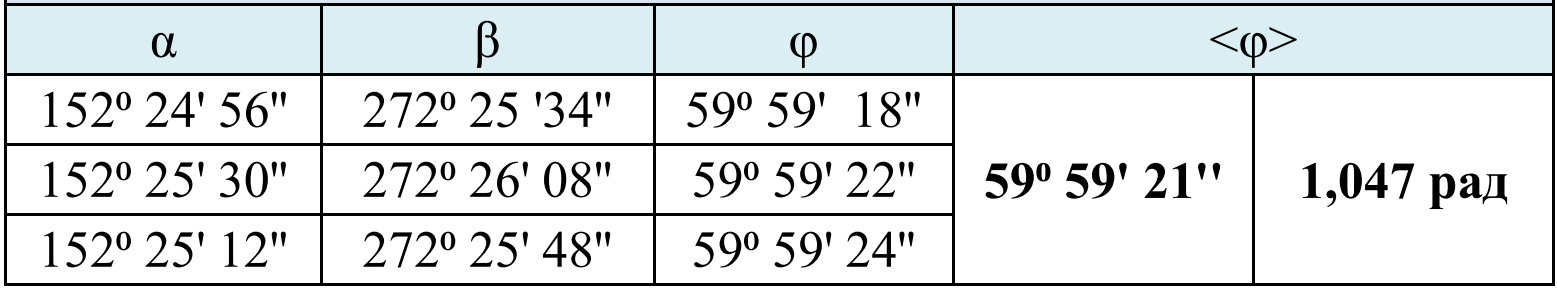
\includegraphics[width=0.8\linewidth]{Pics/tabl1.png}


\label{Teo}

\end{figure}
Усереднюємо і отримуємо радіус кривизни $R = 11,53 м, \epsilon_{R} = 4,4\%$
\subsection{Визначення довжини хвилі червоного скла}
\qquadВважаємо радіус відоомим, тоді отримуємо:

\begin{figure}[ht]

\centering

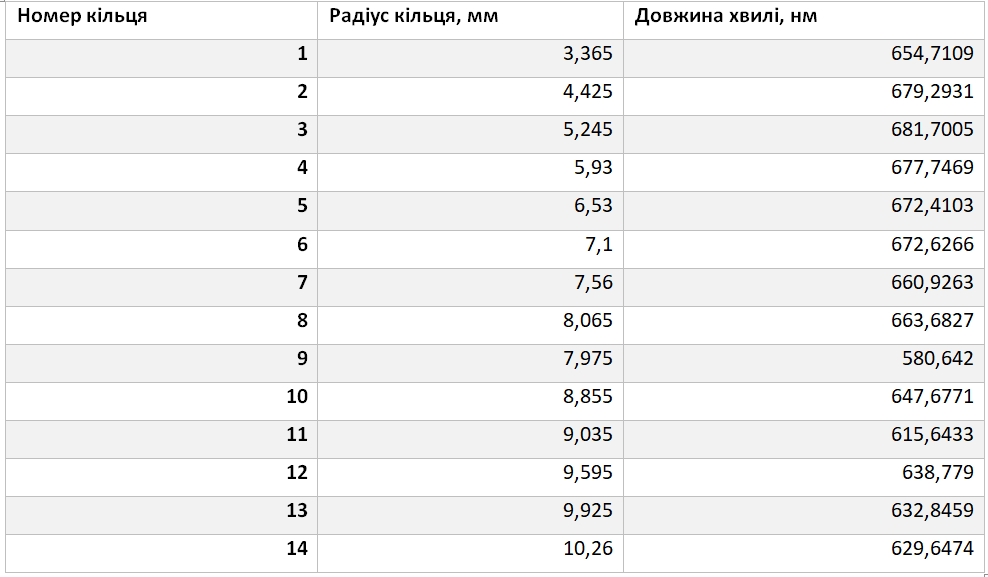
\includegraphics[width=0.8\linewidth]{Pics/tabl2.png}


\label{width}

\end{figure}
Отримані результати для хвилі червоного кольору: $\lambda = 651 нм, похибка \epsilon_{\lambda} = 2,6\%$
\newpage
\subsection{Визначення довжини хвилі синього світла}

\begin{figure}[ht]

\centering

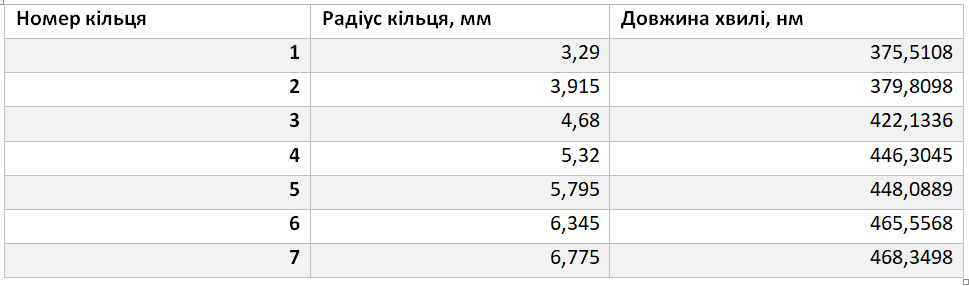
\includegraphics[width=0.8\linewidth]{Pics/tabl3.png}


\label{lenght}

\end{figure}
Отримані результати для хвилі синього кольору: $\lambda = 429 нм, похибка \epsilon_{\lambda} = 8,6\%$
